%! Author = joels
%! Date = 13/07/2021
\section{ASP.NET Theorie}
\subsection{Sonstiges}
\textcolor{b}{\textbf{Convention over configuration:}}\\
Convention over configuration (also known as coding by convention) is a software design paradigm which seeks to decrease the number of decisions that developers need to make, gaining simplicity, and not necessarily losing flexibility. $\rightarrow$ Magie, Schwer anzupassen falls Anforderungen nicht ins Schema passen.\\
\textcolor{b}{\textbf{Multi-Threading:}}
\begin{itemize}[topsep=0pt, leftmargin=3mm]
  \setlength\itemsep{-0.3em}
  \item ASP.NET besitzt einen Thread Pool (Grösse konfigurierbar)
  \item ASP.NET wählt für jeden Request ein Thread aus dem Pool
  \item Thread ist solang blockiert bis der Request abgeschlossen ist
  \item Keine geteilten Daten in Controller und Services halten
\end{itemize}
\textcolor{b}{\textbf{MVVM (Model–View–ViewModel:)}}\\
\textbf{View:} Markup Language, Was Benutzer sieht, Kommunikation zwischen View und ViewModel durch Binding
\textbf{ViewModel:} Daten für View aufbereiten, Value Converter, UI Logik
\textbf{Model:} Daten, Services, Domain Logik\\
\textcolor{b}{\textbf{Middleware:}}\\
Ein Request durchläuft ein Stack von Middlewares (Auf Rückweg kann auch mehr Logik platziert werden). Jede Middleware kann den Request beenden\\
\textcolor{b}{\textbf{Projekt-Struktur:}}\\
\textbf{wwwroot:} Statische Inhalte der Webseite z.B. CSS / JS / HTML
\textbf{appsettings.json:} Einstellungen der Webseite z.B. Connection-String zur DB
\textbf{Programm.cs:} Einstiegspunkt von der Web Applikation
\textbf{Startup.cs:} Konfiguriert die Web App
\subsection{Dependency Injection:}
ASP.NET Core kommt mit einem primitiven Dependency Injection Container. \textbf{Idee:} Klasse erwähnt welche Interfaces benötigt werden. Ein Resolver sucht im Container nach einer geeigneten Klasse und übergibt diese. \textbf{Ziel:} Reduzieren von hoher Kopplung zwischen verschiedenen Klassen.\\
\textcolor{b}{\textbf{Lifetime:}}\\
\textbf{Transient:} Created each time they are requested. Works best for lightweight, stateless services. \textbf{Scoped:} Created once per request. \textbf{Singleton:} Created the first time they are requested. Every subsequent request will use the same instance.\\
\textcolor{b}{\textbf{Captive Dependency Problematik:}}\\
Komponenten dürfen sich nur Komponenten mit gleicher oder längerer Lebensdauer Injection lassen.
\subsection{Pages}
Alternative und vereinfachte Variante vom MVC. Router muss nicht konfiguriert werden. Best-Practices für Serverseitiges-Rendering. \textbf{Kombination mit MVC:} Statische Seiten mit Pages, REST-API mit MVC.\\
\textcolor{b}{\textbf{Routing:}} Bei Aufruf einer URL wird im Folder Pages gesucht $\rightarrow$ Ist case insensitive: \textcolor{b}{/add} rendert \textcolor{b}{/pages/add.cshtml}\\
\textcolor{b}{\textbf{MVVM:}} Pages bestehen aus 2 files: \textbf{*.cshtml:} View mit Razor geschrieben. \textbf{*.cshtml.cs:} View Model. (erbt von PageModel)\\
\textcolor{b}{\textbf{MVVM - Model:}} View Model kann pro HTTP-Verb eine Funktion definieren die davor aufgerufen wird. (z.B. OnGet, OnPost). Dabei werden die Body und Query Parameter automatisch gemappt. $\rightarrow$ Mit [BindProperty] kann auf das Kopieren von Properties verzichtet werden (siehe Code)\\
\textcolor{b}{\textbf{MVVM - View:}} \textbf{@page} definiert das Razor-File als Page. \textbf{@page "/test/\{id?\}"} überschreibt die Default-Routing-Informationen.
\subsection{Razor}
\textcolor{b}{\textbf{Shared/\_Layout.cshtml:}} Generelles Layout der App. Definierst Sections (Placeholders), welche von Page gefüllt werden.\\
\textbf{@RenderBody():} Definiert Platz, wo Content Page rendert.\\
\textbf{@RenderSection():} Definiert Sektion, wo Content Page ihren Inhalt platziert\\
\textcolor{b}{\textbf{\_ViewStart.cshtml:}} Hierarchisch, Code welcher vor Razor-Files ausgeführt wird. Definiert z.B. Layout für alle Pages
\textcolor{b}{\textbf{\_ViewImports.cshtml:}} Hierarchisch, Namespaces / Tag-Helpers können in diesem File registriert werden.\\
\textcolor{b}{\textbf{Tag Helpers:}} Ermöglichen C\# Code an HTML Tags zu binden. Bsp: Email-Tag durch Link Tag ersetzen. $\rightarrow$ Helper müssen im \_ViewImports.cshtml registriert werden\\
\textcolor{b}{\textbf{Partials:}} Markup Files, verwendet innerhalb von anderen Markup Files. Bessere Aufteilbarkeit und Wiederverwendbarkeit.\\
\textcolor{b}{\textbf{View Components:}} Mächtigere Variante von Partials. Beinhalten Logik, können Daten laden/aufbearbeiten. Rendert ein Teil der Seite, Ideal für Ajax (Pages rendern komplette Seite).
\textcolor{b}{\textbf{ViewData/TempData:}} Mit Attribut Gekennzeichnete Daten werden allen Razor-Files im Render-Baum übergeben.\\
\textbf{ViewData/ViewBag:} z.B. Daten an das \_Layout übergeben.\\
\textbf{TempData:} Überlebt ein redirect, Cookie-Middleware nötig.
\subsection{AJAX}
\textcolor{b}{\textbf{Handlers:}} Pages können weitere Actions als handler anbieten.\\
\textbf{Schema:} On[Method][Name]\\
$\rightarrow$ Methoden wie GET/POST/PUT, z.B. OnPostEcho\\
\textbf{Aufruf:} [METHOD]/[Page]?handler=[HandlerName]\\
$\rightarrow$ z.B. POST /Ajax?handler=echo
\subsection{Entity Framework}
Entity Framework (EF) ist eine objektrelationale Zuordnung, die .NET-Entwicklern über domänenspezifische Objekte die Nutzung relationaler Daten ermöglicht. $\rightarrow$ Wenig Code, Viel Konvention, OR-Mapper\\
\textcolor{b}{\textbf{OR-Mapper Idee:}} SQL-Rows auf eine C\# Klasse mappen. Enum-Werte auf ihren Enum-Typen mappen, Relationen auflösen und richtig setzen. \textcolor{b}{\textbf{OR-Mapper Funktionalitäten:}} Umgehen mit Vererbung, Löschen von Einträgen, Migration der Datenbank, Transaktionen. \textcolor{b}{\textbf{Datenbank erstellen:}} Type Discovery (Welche Klassen in die DB), Connection String (Wohin mit Daten), DbContext (Entry Point). \textcolor{b}{\textbf{Wichtige Konventionen:}} \textbf{public [long/string] Id \{get;set;\}:} Wird automatisch zum PK. \textbf{public virtual ApplicationUser Customer \{get;set;\}:} Als Navigation Property erkannt. \textbf{public [long/string] CustomerId \{get;set;\}:} Als FK für Customer Property erkannt. \textcolor{b}{\textbf{Wichtige Attribute:}} \textbf{[Required]:} NotNull in DB. \textbf{[NotMapped]:} Nicht in DB geschrieben. \textbf{[Key]:} Definiert den PK. \textbf{[MaxLength(10)]:} Allokationsgrösse in DB. \textcolor{b}{\textbf{Migration:}} EF Core erlaubt keine automatische Migrationen von Model Änderungen mehr. Nur über Konsole: \textit{dotnet ef database update}
\subsection{Validation}
\textbf{Client-Seitig:} Feedback für User. \textbf{Server-Seitig:} Datenkorrektheit, DB-Infos (z.B. Email schon vergeben)\\
\textcolor{b}{\textbf{Schritt 1: Annotieren der Klassen}}\\
\textbf{Mögliche Attribute:}
\begin{itemize}[topsep=0pt, leftmargin=3mm]
  \setlength\itemsep{-0.3em}
  \item $[$StringLength(60, MinimumLength = 3)$]$
  \item $[$RegularExpression(@"\ldots")$]$
  \item $[$Required$]$
  \item $[$DataType(DataType.Date)$]$
  \item $\rightarrow$ Attribute sind kombinierbar.
\end{itemize}
\textcolor{b}{\textbf{Schritt 2: Razor anpassen}} Validation ins DOM einfügen und JQuery einbinden \textcolor{b}{\textbf{Schritt 3: Server Seitige Validierung}} if (ModelState.IsValid) \{ \ldots \}
\subsection{Authentifizierung}
\textcolor{b}{\textbf{ASP.NET Identity Features:}} PW Stärke, User Validator, Lockout Mechanismus, 2Faktor Auth, Reset PW, OAuth\\
\textcolor{b}{\textbf{ASP.NET Identity Klassen:}} IAuthorizationService (Validation von Policies), UserManager<ApplicationUser>, RoleManager<IdentityRole>, SignInManager\\
\textcolor{b}{\textbf{Aktivierung \& Konfiguration:}} Im Startup.cs \textbf{DI} (services.AddDefaultIdentity<IdentityUser>()) und \textbf{Middleware} (app.UseIdentify()) einbinden. $\rightarrow$ Einstellungen können während der Registration der DI vorgenommen werden z.B. Passwordstärke, Rollenerwartung\\
\textcolor{b}{\textbf{Anwenden: Attribute}}\\
\textbf{[Authorize]:} Benutzer muss authentifiziert sein. Kann auf Controller oder Actions definiert werden. \textbf{[AllowAnonymous]:} Erlaubt für eine spezifische Action anonymen Zugriff.\\
\textcolor{b}{\textbf{Anwenden: User.identity}}\\
\textbf{this.User:} Beinhaltet den eingeloggten User. Type: ClaimsPrincipal $\rightarrow$ Ein Claim ist ein Statement über einen User. Ausgestellt von einem Identity Provider (Role, Name, Email)\\
\textcolor{b}{\textbf{Authentifizierung überprüfen:}}\\
\textbf{Automatisch:} Mit Attribut [Authorize]\\
\textbf{Manuell:} if (User.Identify.IsAuthenticated) \{ \ldots \}
\subsection{Authorisierung}
\begin{lstlisting}[style=csh]
// Lösung 1: Attribute
[Authorize(Roles = "Admin, PowerUser")]
[Authorize(Policy = "OlderThan18, Founders")]
// Lösung 2: Services:
await _userManager.GetUserAsync(User);
await _userManager.IsInRoleAsync(user,"Admin");
// Lösung 3: Claims
User.HasClaim(ClaimTypes.Role, "Admin");
\end{lstlisting}
\textcolor{b}{\textbf{Policy:}} Ermöglichen es, komplexere Regeln zu definieren. z.B. Eine Regel, welche nur für die Founders zutrifft. Oder mehrere Rollen zusammenfassen $\rightarrow$ Man kann auch eigene Regeln wie z.B. unter 18 Jahre definieren.
\subsection{Testing}
3 Varianten von automatisierten Tests: \textbf{Unit, Controller und Integration Tests}\\
Ein Unit Test muss mit dem Attribut \textbf{[Fact]} gekennzeichnet werden. Wie Testet man Magie (z.B. Handlers)? $\rightarrow$ Validation in Test Methode manuell ausführen\\
\textcolor{b}{\textbf{Datenbank:}} Nicht auf echter Datenbank testen. Gründe: Multi-Threading, Inhalt nicht immer bekannt, nicht performant. \textbf{Lösung:} In Memory DB oder DbContext Mocken
\subsection{API Routing}
Services und Endpoints müssen im Startup.cs registriert werden. Das Routing funktioniert über Atrribute:\\
\textbf{[Route]:} Auf Klasse, definiert neuen Eintrag im Router\\
\textbf{[HttpMethod]:} Auf Methode, bei Actions.\\
\begin{minipage}{0.5\linewidth}
  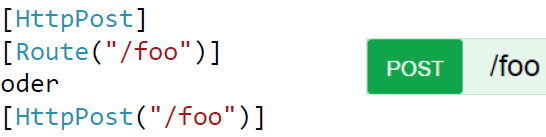
\includegraphics{asp_routing_1.png}
\end{minipage}
\begin{minipage}{0.5\linewidth}
  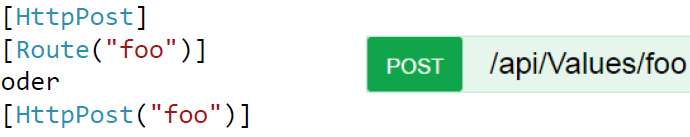
\includegraphics{asp_routing_2.png}
\end{minipage}
\subsection{Swagger, Rest HATEOAS, Exception Handling, JWT}
\textcolor{b}{\textbf{Swagger:}} Eine Spezifikation für die Dokumentation von REST APIs. Programmiersprachen unabhängig. Wird im \textit{Startup.cs} eingetragen. Default unter \textit{http://[server-name]/swagger} erreichbar. $\rightarrow$ C\# ermöglicht es Kommentare als XML zu exportieren. Dieses kann von Swagger angezogen werden, um die API zu beschreiben. Alternativen: RAML, GraphQL\\
\textcolor{b}{\textbf{REST HATEOAS:}} Verlinkte Daten als Links zu Verfügung stellen.\\
\textcolor{b}{\textbf{Exception Handling:}} Error Handling soll generisch funktionieren. $\rightarrow$ Vorgehen: Es gibt eine Exception, welche die notwendigen Daten sammelt. Es gibt einen globalen Errorhandler, welcher diese Exception für Client aufbereitet. Bei einem ungültigen Zustand wird Custom-Exception ausgelöst.\\
\textcolor{b}{\textbf{JWT:}} Übertragen bei Request im http-header. Aufbau: Header, Payload (Claims), Signatur. ASP.NET bietet Middleware für Token Validierung (z.B. JwtBearerMiddleware). Token nur über https versenden: app.UseHttpsRedirection(); app.UseHsts();
\section{ASP.NET Code}
\subsection{Simple BMI Rechner}
\begin{lstlisting}[style=csh]
// Startup.cs
public void ConfigureServices(...) {
  services.AddMvc();
  services.AddSingleton<IBmiService, BmiService>(); }
public void Configure(...) {
  app.UseEndpoints(endpoints => {
    endpoints.MapRazorPages(); }); }

// Data/Bmi.cs (Modell)
public class Bmi {
  [Range(0, 300)]
  [Display(Name = "Gewicht in kg")]
  public double Weight { get; set; }

  [Range(30, 250)]
  [Display(Name = "Höhe in cm")]
  public double Height { get; set; } }

// Services/BmiService.cs
public interface IBmiService {
  double Calculcate(Bmi data); }

  public class BmiService : IBmiService {
    public double Calculcate(Bmi data) {
      return Math.Round(data.Weight + data.Height } }
// Pages/Bmi.cshtml.cs
public class BmiModel : PageModel {
  private readonly IBmiService _bmiService;
  public BmiModel(IBmiService bmiService) {
    _bmiService = bmiService; }

  [BindProperty(SupportsGet = true)]
  public Bmi Bmi { get; set; }

  public bool WrongData { get; set; }
  public double BmiValue { get; set; }

  public void OnGet() {
    if (ModelState.IsValid) { BmiValue = _bmiService.Calculcate(Bmi); }
    else { WrongData = true; } } }
// Pages/Bmi.cshtml
@page
@model BmiRechner.Pages.BmiModel
@{ ViewData["Title"] = "Bmi"; Layout = null; }
@if (Model.WrongData) {
  <p>Wrong Data</p> } else {
  <p>@Model.BmiValue</p> }
// Pages/Index.cshtml.cs
public class IndexModel : PageModel {
  public Bmi Bmi { get; set; } = new Bmi(){Height =170, Weight = 80}; // Startdata
  public void OnGet() { ... } } // OnPost()
// Pages/Index.cshtml
@page
@model IndexModel
@{ ViewData["Title"] = "Home page"; }
<form asp-page="Bmi"data-ajax="true" data-ajax-method=
"GET" data-ajax-mode="replace" data-ajax-update="#res">
  <input asp-for="@Model.Bmi.Height" name="height">
</form> <div id="res"></div>
\end{lstlisting}
\subsection{BMI API}
\begin{lstlisting}[style=csh]
// Startup.cs
endpoints.MapControllers();
// Controllers/BmiController.cs
[Route("api/[controller]")]
[ApiController]
public class BmiController : ControllerBase {
  private readonly IBmiService _bmiService;
  public BmiController(IBmiService bmiService) {
    _bmiService = bmiService; }

  [HttpGet] // HttpPost -> [FromBody]
  public double Calculate([FromQuery] Bmi data) {
    return _bmiService.Calculcate(data); } }
\end{lstlisting}